\documentclass[a4paper, 12pt]{article}
\usepackage{ctex} %使文档可以输入中文
\usepackage{amsfonts}
\usepackage{float}
\usepackage{graphicx}
\usepackage{amsmath,amssymb,amsfonts}
\begin{document}
    \title{黑洞渲染器}
    \maketitle
    \section{简介}
    电影《星际穿越》中名为“卡冈图雅”的黑洞给了我很大的震撼,从第一次看到它我就想自己复现一遍。在24秋期末
    看到有一个别的团队做了一个效果不错的,这让我重新想起之前的计划,于是25春选了计算机图形学、开始
    自己看广义相对论,准备完成这个项目。感谢大作业给了我一个这样的机会(不然可能拖到暑假自己
    慢悠悠地做了)。

    本项目主要使用cpp编写,采用CMake构建,调用库包含Eigen、GLAD、GLFW、ImGui、GSL以及Matplotlibcpp。最后两个
    主要用于测试(GSL为了显示氢原子的轨道以测试体渲染,Matplotlibcpp以测试测地线方程求解器)。以及部分glsl语言实现
    渲染等效果。项目也包含了
    部分python语言编写的符号计算程序(用于计算任意时空下的联络以便计算测地线)。

    本项目使用的环境是VSCode,CMake配置使用Visual Studio Community 2022 Release - amd64.
    如果您在运行GEODESIC\underline \ TEST或\\GEODESIC\underline \ AUTO\underline \ TEST项目,请确保
    您的环境中存在python以及numpy.
    \section{项目内容}
    本项目最终要实现黑洞及其吸积盘的渲染。
    \subsection{测地线计算}
    在广义相对论下,时空是一个定义了度规的四维流形,物体不受其他作用时的运动轨迹是
    四维流形上的一条测地线(而光对应的测地线上的切矢量长度恒为0)。测地线方程如下:
    \begin{align*}
        \frac{\mathrm d^2 x^{\mu}}{\mathrm d \lambda ^2} = {\Gamma^{\mu}}_{\nu\eta}\frac{\mathrm d x^{\nu}}{\mathrm d \lambda}\frac{\mathrm d x^{\eta}}{\mathrm d \lambda} ,\mu = 0,1,2,3 
    \end{align*}
    \par 切矢为零的条件如下:
    \begin{align*}
        g_{\mu\nu}v^{\mu}v^{\nu} = 0
    \end{align*}
    对于最简单的黑洞——施瓦西黑洞,其周围的时空是球对称的,因此每一束光经过其的轨迹都可以
    简单地在过黑洞中心的一个平面上计算。考虑用$r(\lambda),\theta(\lambda) = \frac{\pi}{2} ,\phi(\lambda),t(\lambda)$
    计算,则化简后得到:
    \[\frac{\mathrm d^2 }{\mathrm d \phi^2}(\frac{1}{r} )= -\frac{1}{r} + 3 M (\frac{1}{r} )^2 \]
    本项目直接采用半隐式欧拉法进行数值求解。
    \subsection{体渲染}
    仅考虑吸积盘的发光和散射,不考虑星光,原因是星光的相对强度太低(类似于观测太阳就看不到星星)。
    那么直接使用体渲染公式:
    \begin{align*}
        I = \int_{0}^{S}P(x)\exp[-\int_0^x \alpha(t) \mathrm d t]\mathrm d x
    \end{align*}
    P(x)是$x$处吸积盘三通道发光功率密度,$\alpha(x)$是x处对光的吸收率。公式中不考虑多散射和背景光。
    \subsection{黑体辐射}
    从$https://www.freesion.com/article/8583280768/$中借鉴了温度到RGB三通道颜色的算法(实际上
    更正确的做法可能需要转换为XYZ坐标,这是未来的改进方向之一)。
    目前还考虑了伽马校正,先将颜色各分量作2.2次方,叠加后再作1/2.2次方。
    \subsection{吸积盘噪声}
    \subsubsection{Perlin噪声}
    Perlin噪声是在每个整数点$\mathbf u_i$上给定一个梯度向量$\mathbf v_i$,然后每个$\mathbf x$上的取值通过:
    \par
    1.通过一个连续的坐标变换A变换到$\mathbf y$ \par
    2.计算:
    \[\sum_{i} f(\mathbf y,\mathbf u_i)(\mathbf y - \mathbf u_i)\cdot \mathbf v_i \]
    $u_i$是$\mathbf y$附近的整数点,$f(\mathbf y,\mathbf u_i)$是权函数。将结果作为$\mathbf x$处的噪声强度$perlin(\mathbf x)$。
    \subsubsection{旋转吸积盘}
    将时间$t$传入shader,于是每次计算$\mathbf x$处的密度函数就采用:
    \[perlin(\mathbf A(\mathbf x,t))\]
    其中A是一个变换,用于寻找$x$位置处的吸积物质在$t$时刻前处于什么位置。这里处理地非常简单,直接
    使用$A$为一个仅于$|x|$有关的旋转变换(不同位置有不同的角速度)。施瓦西时空下物质转速是:
    \begin{align*}
        v(r) = \sqrt{\frac{GM}{r - r_s}}
    \end{align*}
    其中$r_s = 2M$\par
    \subsubsection{双盘叠加}
    由于不同位置角速度不同,旋转久了会产生扭曲,于是我借鉴了$https://zhuanlan.zhihu.com/p/20536269771$
    的方法,即用两个吸积盘叠加。我采取的方式是:
    \par
    对于盘1,其强度正比于$\sin^2 \pi (kt-\mathrm{floor}(kt))$,其用于计算吸积盘的t代为:
    $t-\frac{1}{k}\mathrm{floor}(kt)$
    \par
    对于盘2,其强度正比于$\cos^2 \pi (kt-\mathrm{floor}(kt))$,其用于计算吸积盘的t代为:
    $t-\frac{1}{k}\mathrm{floor}(kt-0.5)$  \par
    这样,两个盘在相位突变的时候强度都为0,叠加总强度为1,视觉效果较好。
    \subsection{多普勒效应}
    对于同一个运动的物体,不同位置观测者观测到的光频率、强度均不同。
    相对论下运动物体辐射强度、频率和其本征参考系下的强度、频率之间关系:
    \begin{align*}
        I = \frac{I_0}{\gamma^4(1+\beta\cos\theta)^4}
    \end{align*}
    \begin{align*}
        \nu = \frac{\nu_0}{\gamma(1+\beta\cos\theta)}
    \end{align*}
    再结合黑洞积吸盘某处的转速:
    \begin{align*}
        v(r) = \sqrt{\frac{GM}{r - r_s}}
    \end{align*}
    其中$r_s = 2M$\par
    考虑之前的黑体辐射公式,温度的变化比与$\gamma$的变化比相同.
    \subsection{泛光}
    先提取高亮的部分.这里为了防止突变,我将低亮部分也取了一部分(采取权值为$(\frac{p}{p_0} )^k,p_0$是临界值)。
    之后利用横向高斯卷积和纵向高斯卷积交替进行(如果直接采用二维卷积核,那么每次卷积计算量为$N^2$,现在这样
    做每次计算量为$2N$).
    \subsection{其他时空下的测地线}
    平直时空下线元长度表达式:
    \[\mathrm ds^2 = -\mathrm dt^2 +\mathrm dr^2 + r^2\mathrm d\theta^2 + r^2\sin^2 \theta \mathrm d\phi ^2\]
    之前采用的施瓦西时空,其中线元长度表达式为:
    \[\mathrm ds^2 = -(1-\frac{2M}{r} )\mathrm dt^2 +(1-\frac{2M}{r} )^{-1}\mathrm dr^2 + r^2\mathrm d\theta^2 + r^2\sin^2 \theta \mathrm d\phi ^2\]
    这说明其是球对称的,因此其很容易化为一个仅与$r-\phi$相关的微分方程,很容易求解。
    而旋转不带电黑洞产生的时空(Kerr时空)中的线元长度表达式为:
    \begin{align*}
    ds^2 =& -\left(1 - \frac{2Mr}{\rho^2}\right) dt^2 + \frac{\rho^2}{\Delta} dr^2 + \rho^2 d\theta^2\\
        & + \left(r^2 + a^2 + \frac{2Mr a^2 \sin^2 \theta}{\rho^2}\right) \sin^2 \theta \, d\phi^2 - \frac{4Mr a \sin^2 \theta}{\rho^2} dt \, d\phi
    \end{align*}
    其中:
    \[\rho^2 = r^2 + a^2 \cos^2 \theta, \ \ \Delta = r^2 - 2Mr + a^2. \]
    \par 接下来我们面临两个困难:
    \par 1.线元形式峥嵘而崔嵬,而联络有64个,每个的计算式:
    \[
    \Gamma^\lambda_{\mu\nu} = \frac{1}{2} g^{\lambda\rho} \left( \partial_\mu g_{\nu\rho} + \partial_\nu g_{\mu\rho} - \partial_\rho g_{\mu\nu} \right)
    \]
    虽然联络具有对称性$\Gamma^{\mu}_{\ \nu \gamma} = \Gamma^{\mu}_{\  \gamma\nu}$,我们也要至少计算
    32次上面的式子。无论如何,对如此复杂的度规求两位数次数的偏导、矩阵乘,在计算上是很难的。
    \par
    2.在球坐标下,我们在$\sin \theta = 0$时会遇到奇点,如果数值方法较差我们会面临困难。而且,球坐标的不均匀性可能需要
    我们采用自适应的步长...总之由球坐标带来的困难很多。
    \par
    我采用的解决方法如下:\par
    问题1:通过python的sympy库进行符号计算,然后用其ccode功能把符号计算结果导出到$.h$的cpp头文件。\par
    问题2:解决方案是在笛卡尔坐标系$Oxyz$下进行计算。但是我们没有直接计算由xyz显示确定的联络,而是计算了
    由$r,\theta,\phi,t$给定的非平直时空球坐标联络(直接在xyzt下符号计算及其费时),再减去平直时空在$r,\theta,\phi,t$下的联络得到$\widetilde{\Gamma}$ .
    可以证明,$x,y,z,t$对$\lambda$的二阶导,可以直接通过由假联络$\widetilde{\Gamma}$在$r,\theta,\phi,t$
    下计算的坐标的二阶导坐标变换回来(把计算得到的$(r'',\theta'',\phi'',t'')$当作矢量)。
    (如果直接用球坐标下的联络计算,我们还需要面临坐标变换带来的加速度。这里取假联络实际上相当于
    用平直时空联络全0的特征把坐标变换带来的加速度消掉了。)
    \section{实现流程}
    \subsection{测地线测试GEODESIC\underline \ TEST}
    本项目主要用于检测头文件"geodesic.h"(用于计算施瓦西时空下的测地线)。
    %TODO:引入/photo下的geodesic_test.png
    \par 
    \begin{figure}[H]
        \centering
        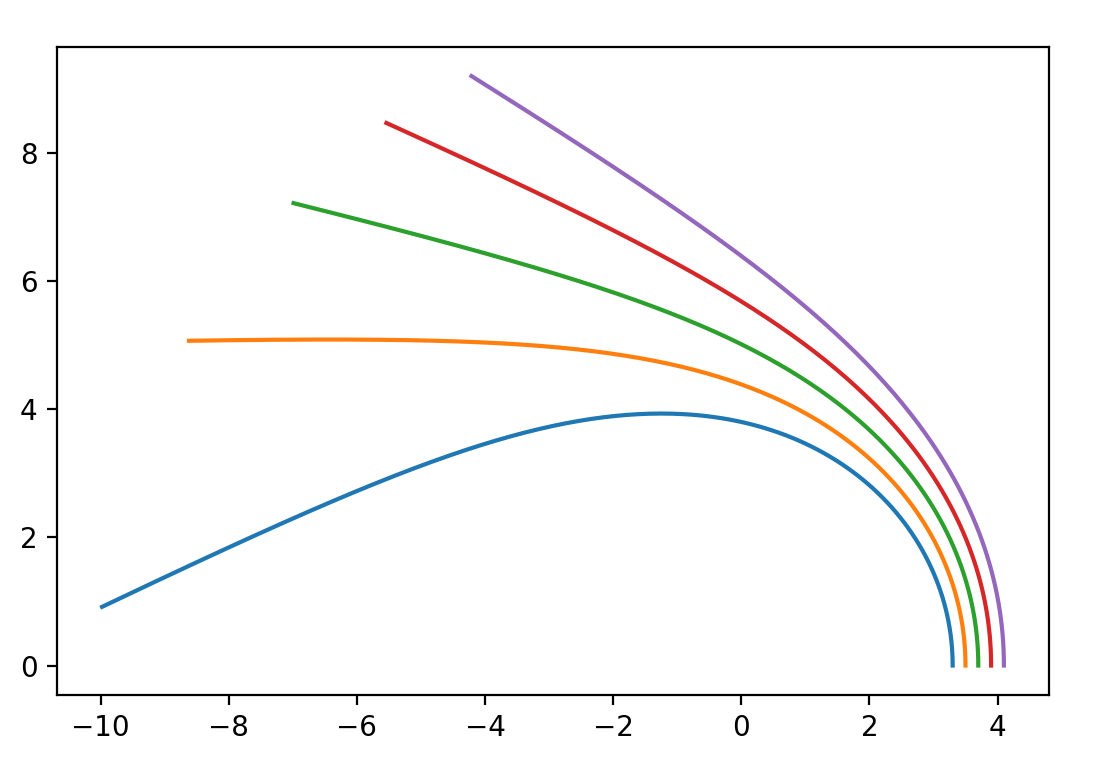
\includegraphics[width=0.55\textwidth]{photo/geodesic_test.png}
        \caption{类光测地线测试结果,其中黑洞半径R=2}
    \end{figure}
    
    
    \subsection{体渲染测试VOLUME\underline \ R}
    在cpu中实现了体渲染流程(volume\underline \ render.cpp),用GSL计算了氢原子的轨道密度函数并显示(使用平直时空下的步进Flat\underline \ ST\underline \ RayMarch)。
    \begin{figure}[H]
    \centering
    \begin{minipage}[t]{0.48\textwidth}
        \centering
        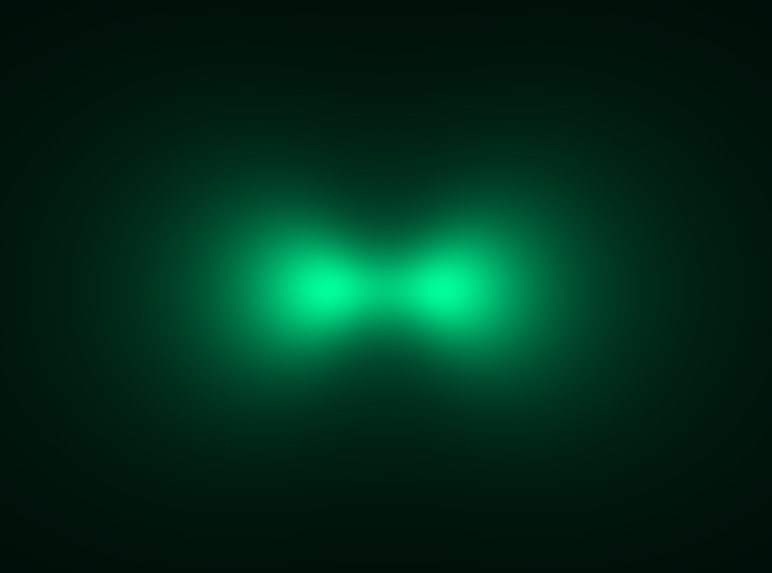
\includegraphics[width=0.95\textwidth]{photo/322x025.png}
        \caption{主/角/磁量子数3/2/2}
    \end{minipage}
    \hfill
    \begin{minipage}[t]{0.48\textwidth}
        \centering
        
\includegraphics[width=0.95\textwidth]{photo/321x025.png}
        \caption{主/角/磁量子数3/2/1}
    \end{minipage}
\end{figure}
    之后用Schwarzschild\underline \ BH\underline \ RayMarch类(用到了geodesic.h)
    初步计算了施瓦西黑洞的效果。
    \begin{figure}[H]
        \centering
        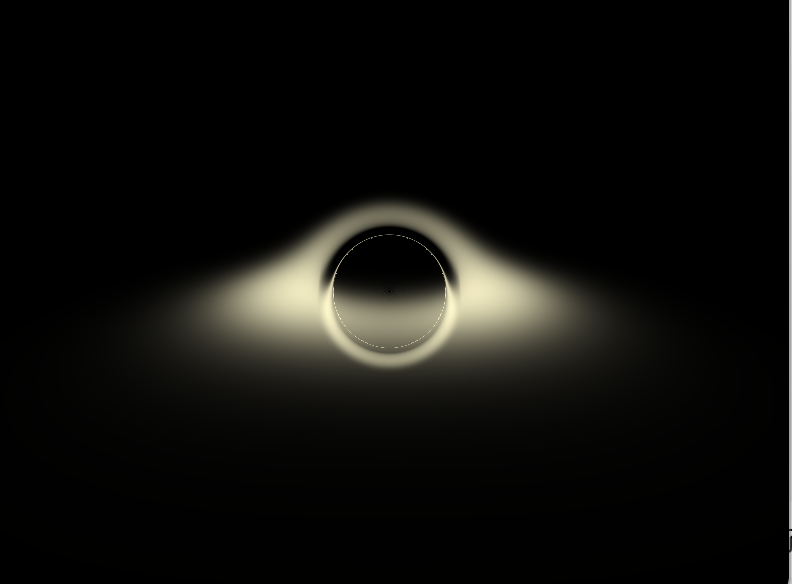
\includegraphics[width=0.95\textwidth]{photo/Swz_BH_1.png}
        \caption{带褐色吸积盘的施瓦西黑洞}
    \end{figure}
    此时成图颇具廉价感。从现在的角度来说:缺少泛光、吸积盘没有噪声、颜色不正确。
    \subsection{CPU上的泛光}
    为了方便测试、兼容之前的工作,我决定现在CPU上实现泛光。
    一开始直接使用二维高斯核进行卷积,但效率感人。后来用横纵一维卷积交叠代替了高斯卷积,效率逐渐可以接受。
    (直到此时,所有工作成果都不是实时的,要花很长时间渲染一张图)。
    再略调了调颜色使吸积盘变成橙色后、,得到了如下结果:
    \begin{figure}[H]
        \centering
        % 第一行
        \begin{minipage}[t]{0.48\textwidth}
            \centering
            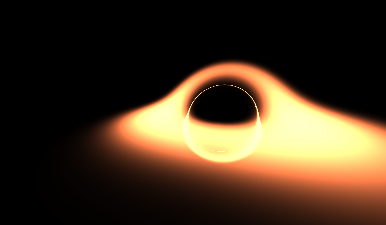
\includegraphics[width=0.95\textwidth]{photo/bloom0.png}
            \caption{效果图1}
        \end{minipage}
        \hfill
        \begin{minipage}[t]{0.48\textwidth}
            \centering
            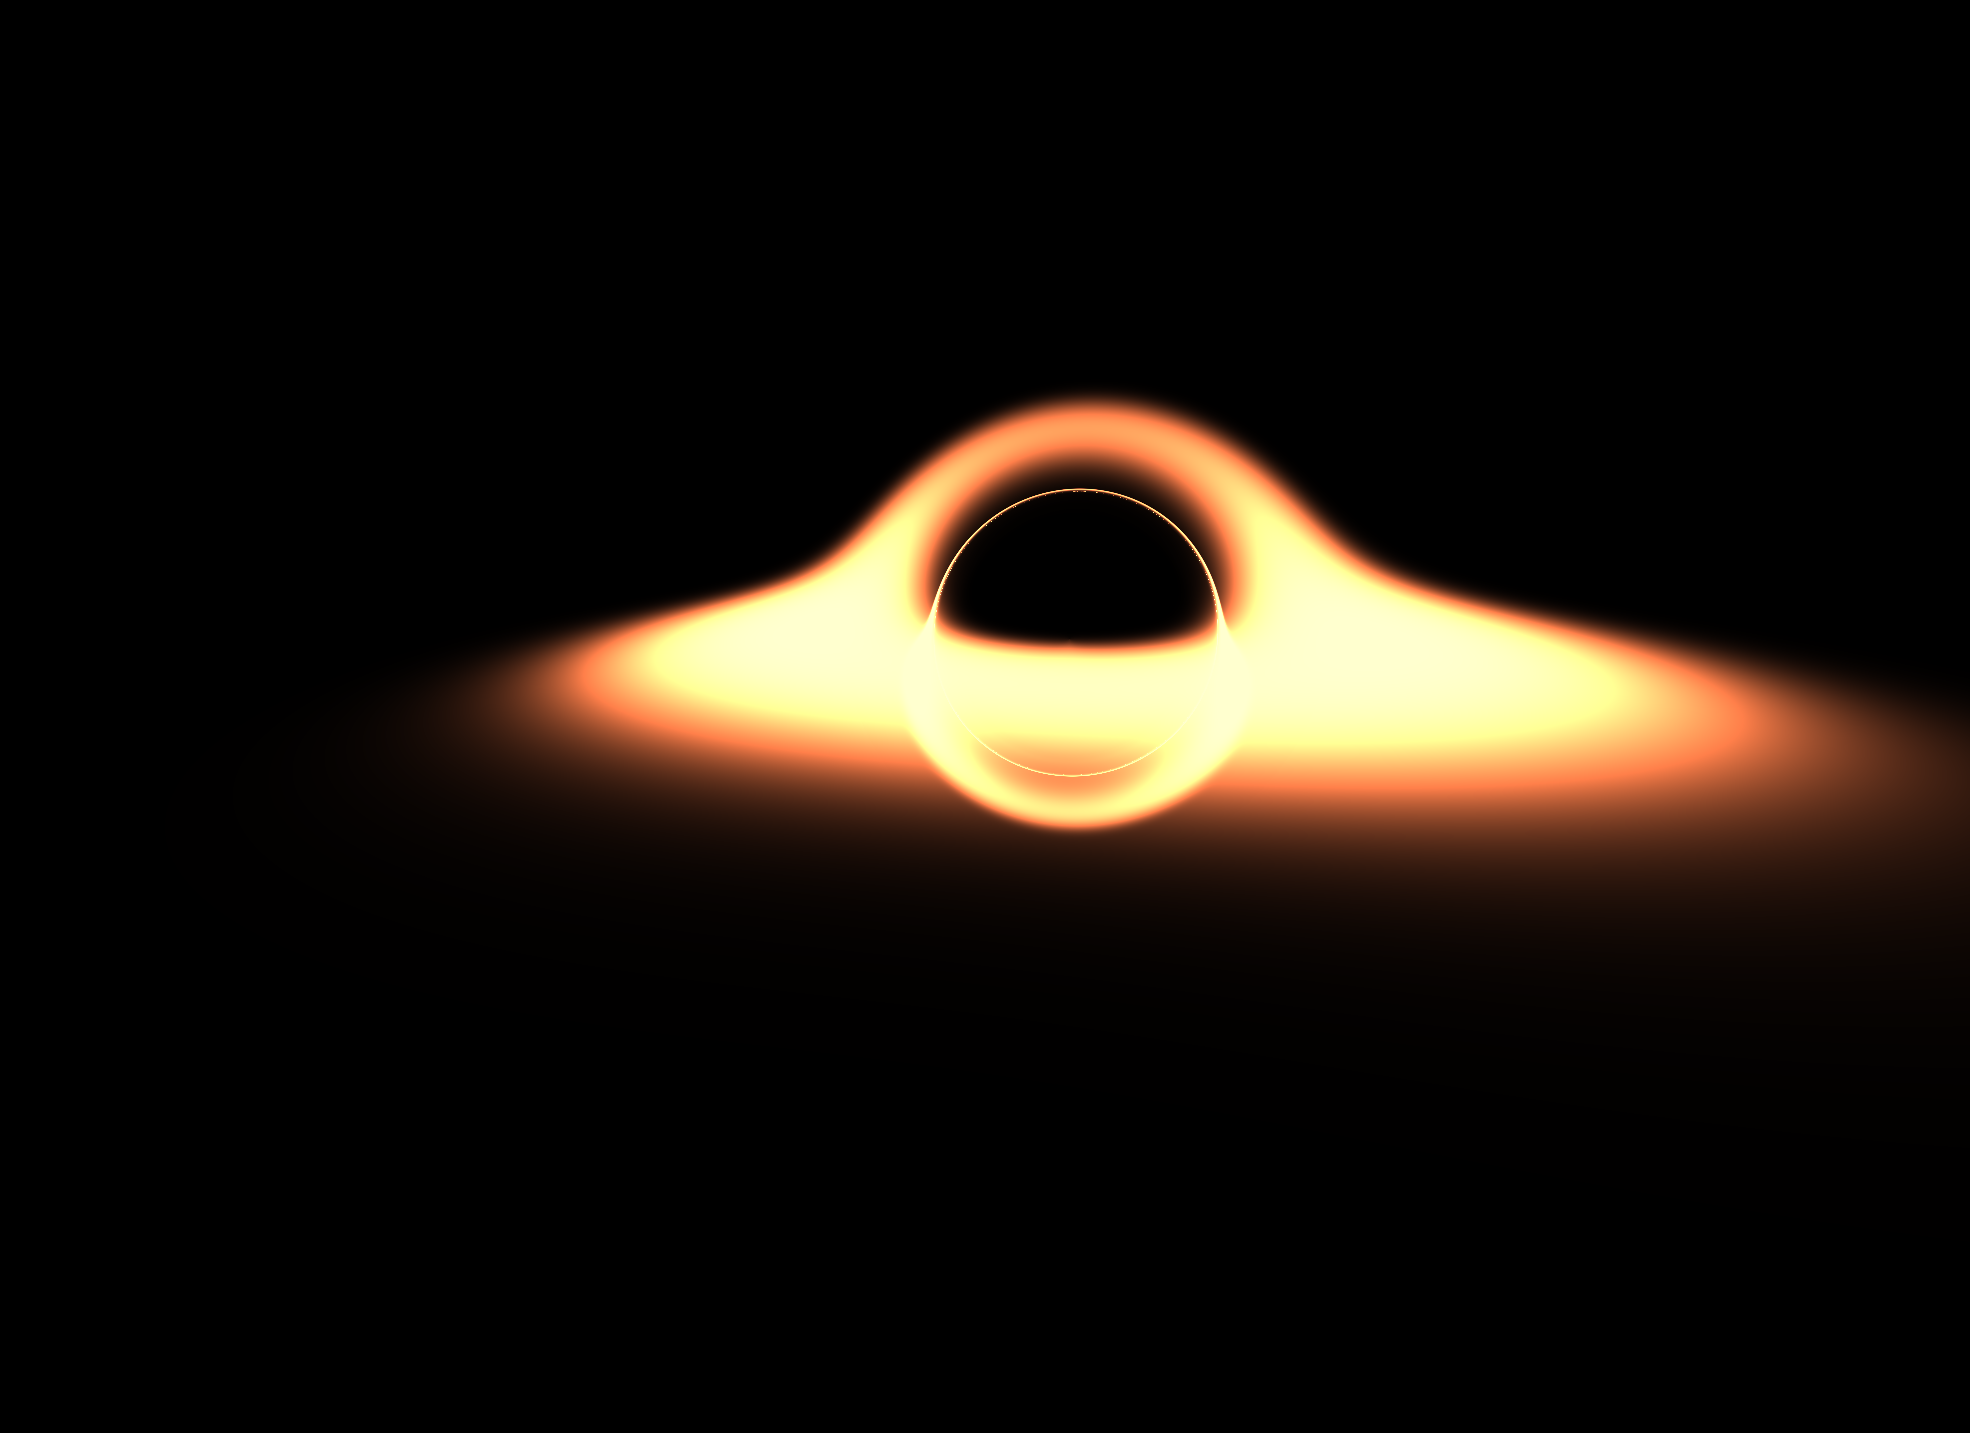
\includegraphics[width=0.95\textwidth]{photo/bloom1.png}
            \caption{效果图2}
        \end{minipage}
        \vskip\baselineskip
        % 第二行
        \begin{minipage}[t]{0.48\textwidth}
            \centering
            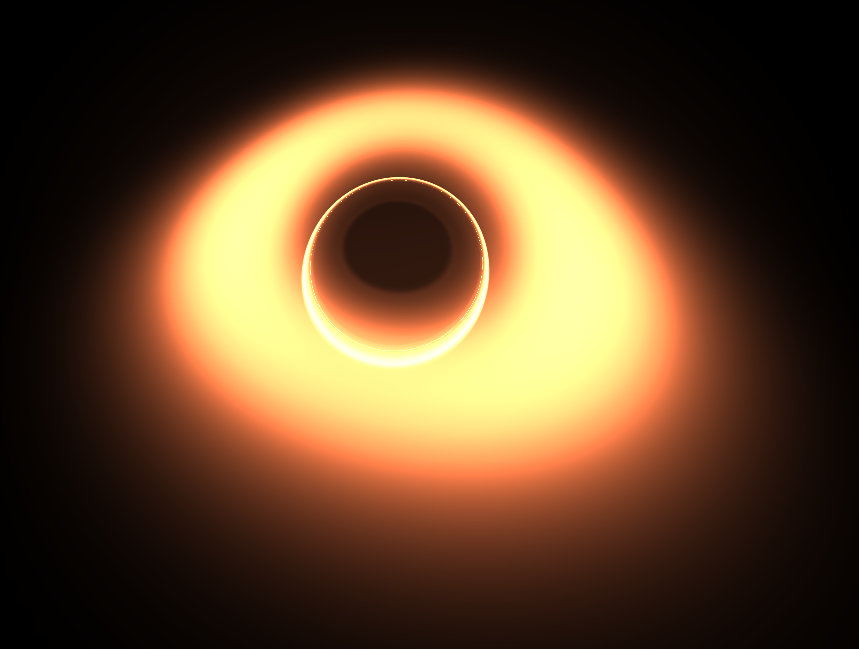
\includegraphics[width=0.95\textwidth]{photo/bloom2.png}
            \caption{效果图3}
        \end{minipage}
        \hfill
        \begin{minipage}[t]{0.48\textwidth}
            \centering
            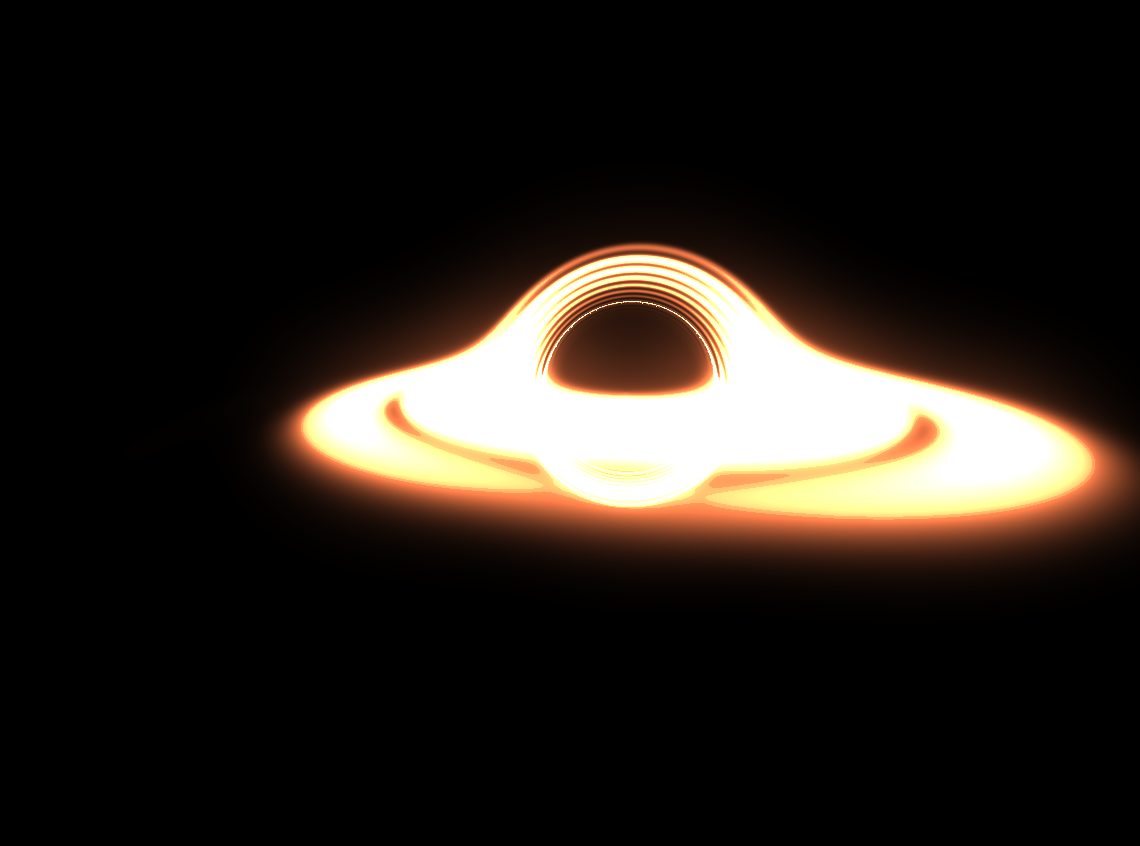
\includegraphics[width=0.95\textwidth]{photo/bloom3.png}
            \caption{效果图4(在吸积盘函数中加了和r相关的正弦函数,另外泛光有点过高了)}
        \end{minipage}
    \end{figure}
    \subsection{初步并行、吸积盘噪声、光强多普勒效应}
    这里抛弃了Volume\underline \ Render.h,开始使用opengl的compute shader进行体渲染。
    添加了吸积盘噪声(使用Perlin噪声),并且添加了光强多普勒效应。
    \begin{figure}[H]
        \centering
        % 第一行
        \begin{minipage}[t]{0.48\textwidth}
            \centering
            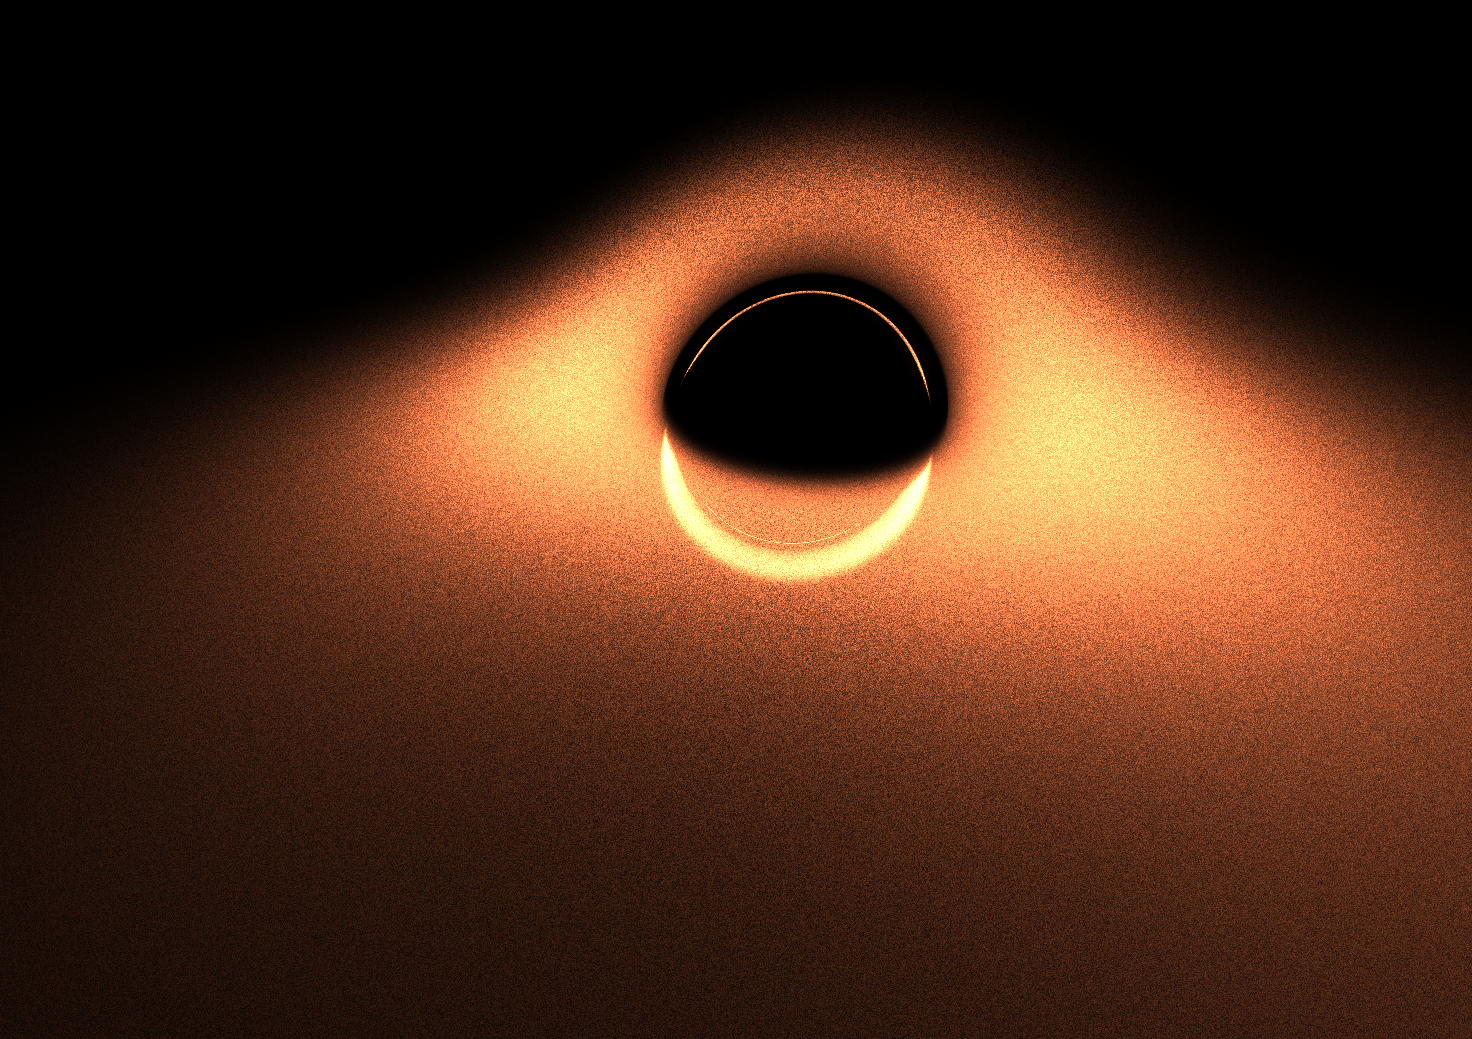
\includegraphics[width=0.95\textwidth]{photo/perlin2.png}
            \caption{效果图1(无多普勒,细噪声)}
        \end{minipage}
        \hfill
        \begin{minipage}[t]{0.48\textwidth}
            \centering
            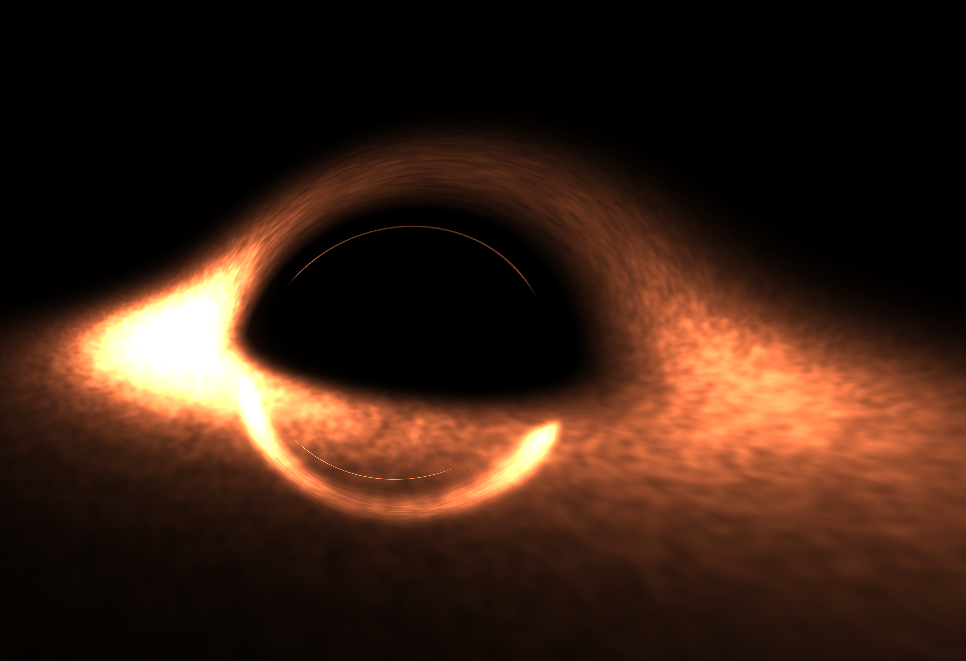
\includegraphics[width=0.95\textwidth]{photo/perlin0.png}
            \caption{效果图2(光强多普勒,粗噪声)}
        \end{minipage}
        \hfill
        \begin{minipage}[t]{0.48\textwidth}
            \centering
            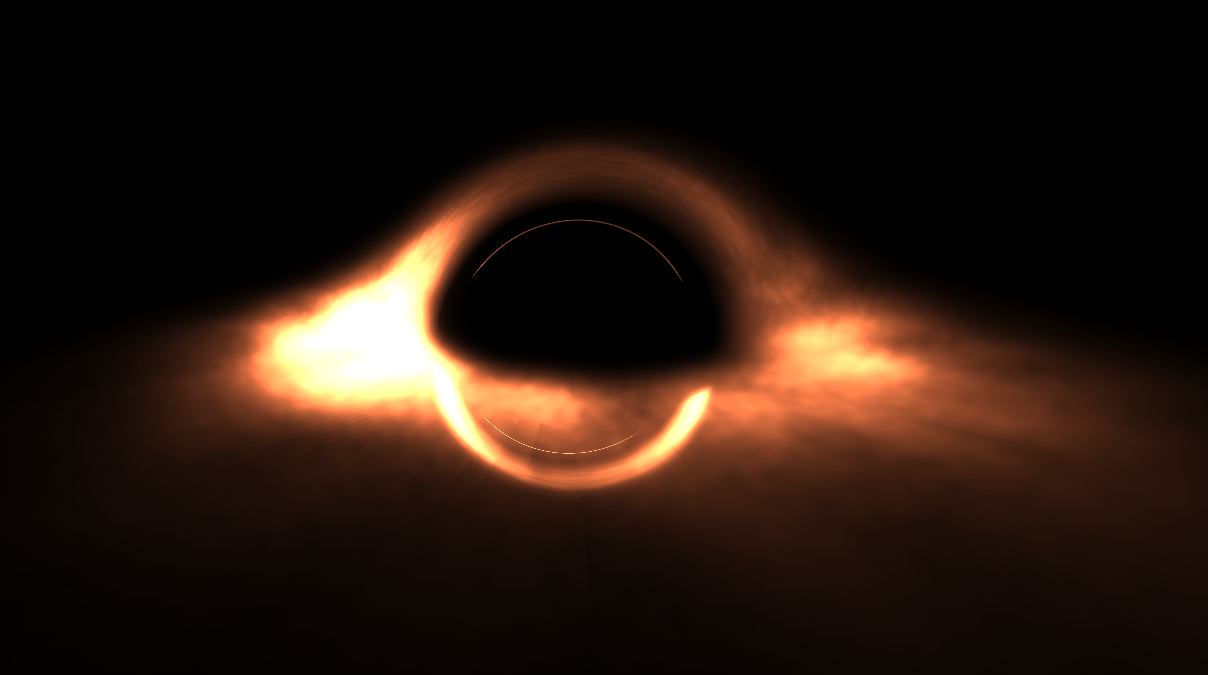
\includegraphics[width=0.95\textwidth]{photo/perlin1.png}
            \caption{效果图3(光强多普勒,粗噪声)}
        \end{minipage}
        \hfill
        % 第二行
        \begin{minipage}[t]{0.48\textwidth}
            \centering
            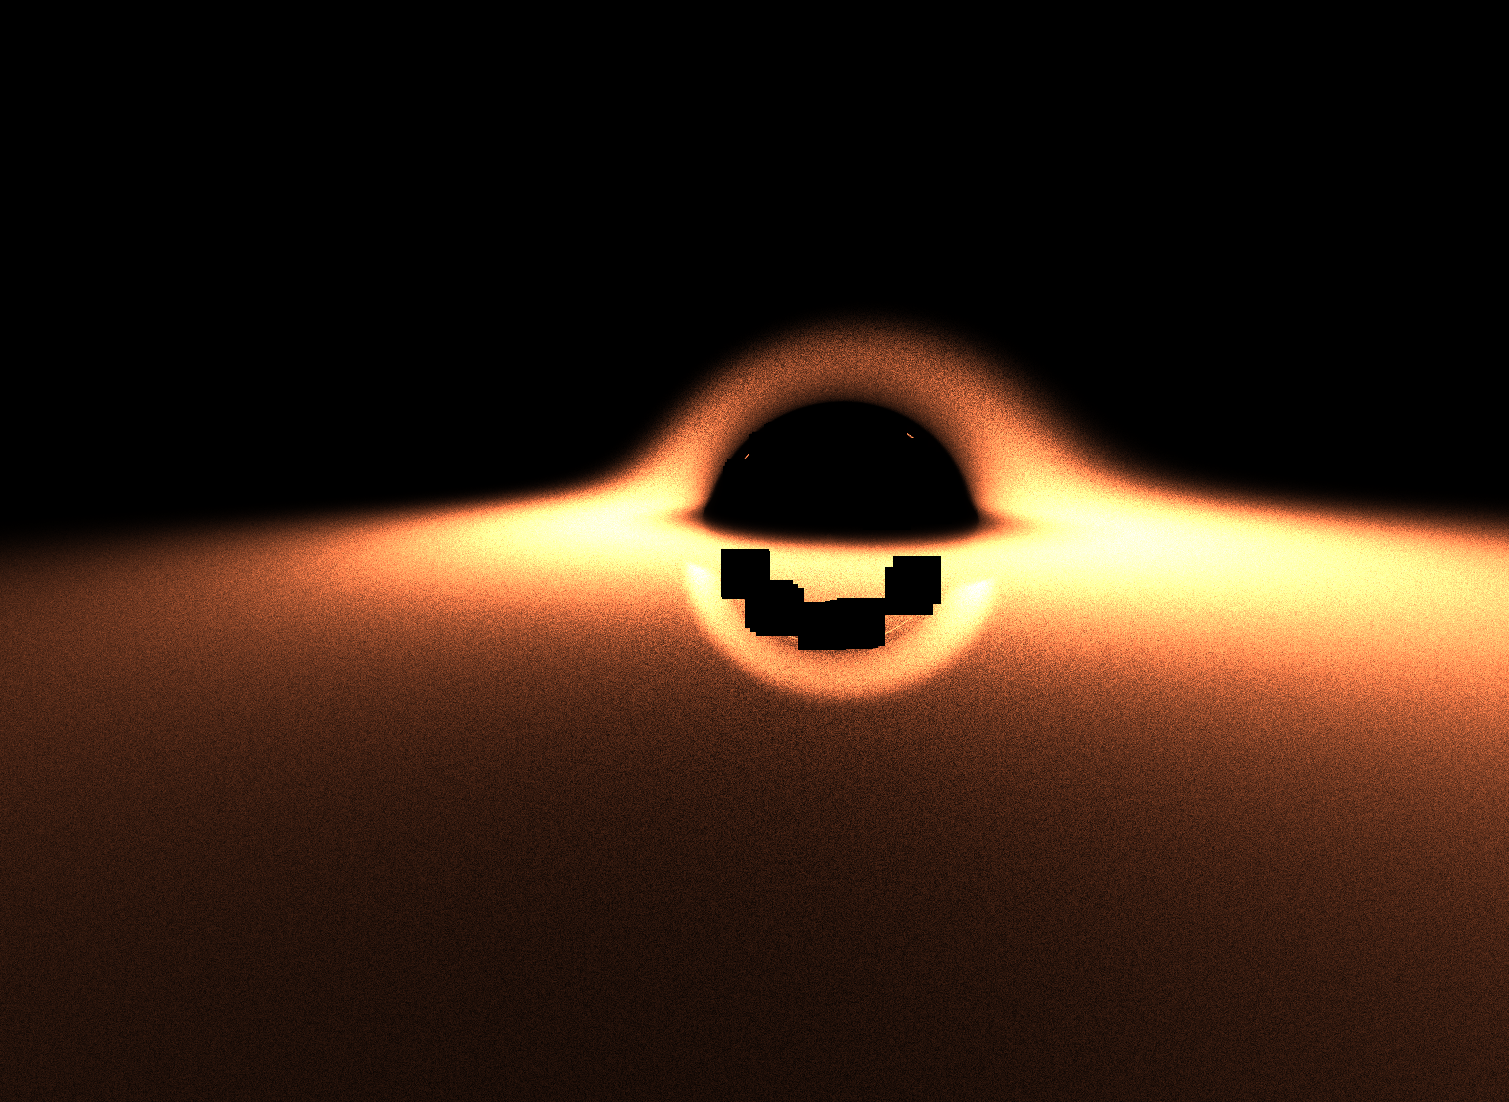
\includegraphics[width=0.95\textwidth]{photo/bug0.png}
            \caption{遇到的小bug(似乎是雾生成时对负数进行了开跟)}
        \end{minipage}
        
    \end{figure}
    \subsection{温度-RGB转换、频率多普勒、泛光GPU化}
    在之前的compute shader中添加了温度到RGB的转换以及频率的多普勒效应。
    之后将泛光的计算也移到了GPU上。
    \begin{figure}[H]
        \centering
        % 第一行
        \begin{minipage}[t]{0.48\textwidth}
            \centering
            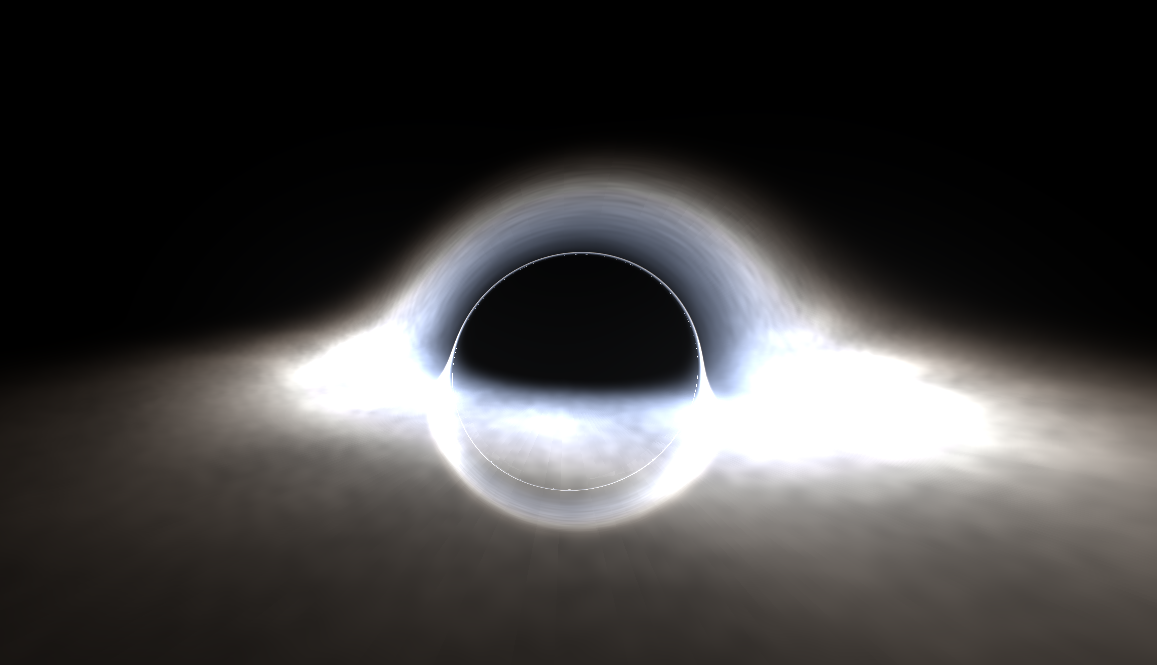
\includegraphics[width=0.95\textwidth]{photo/gb0.png}
            \caption{效果图1(无多普勒)}
        \end{minipage}
        \hfill
        \begin{minipage}[t]{0.48\textwidth}
            \centering
            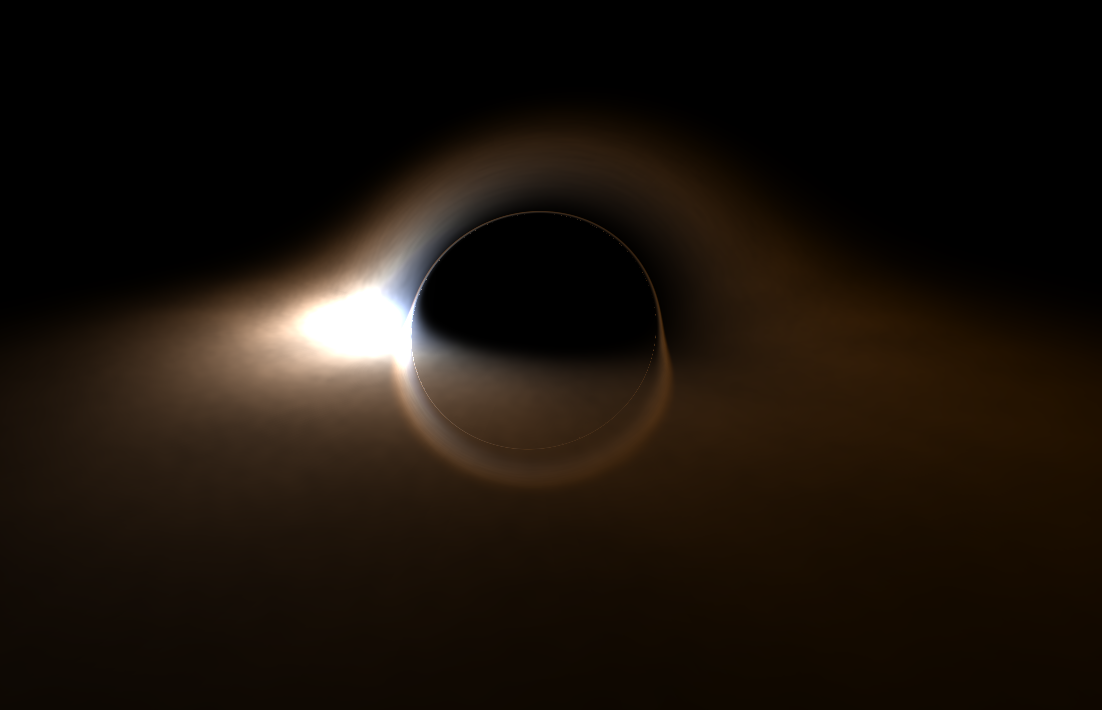
\includegraphics[width=0.95\textwidth]{photo/gb1.png}
            \caption{效果图2(双多普勒)}
        \end{minipage}
        \hfill
        \begin{minipage}[t]{0.48\textwidth}
            \centering
            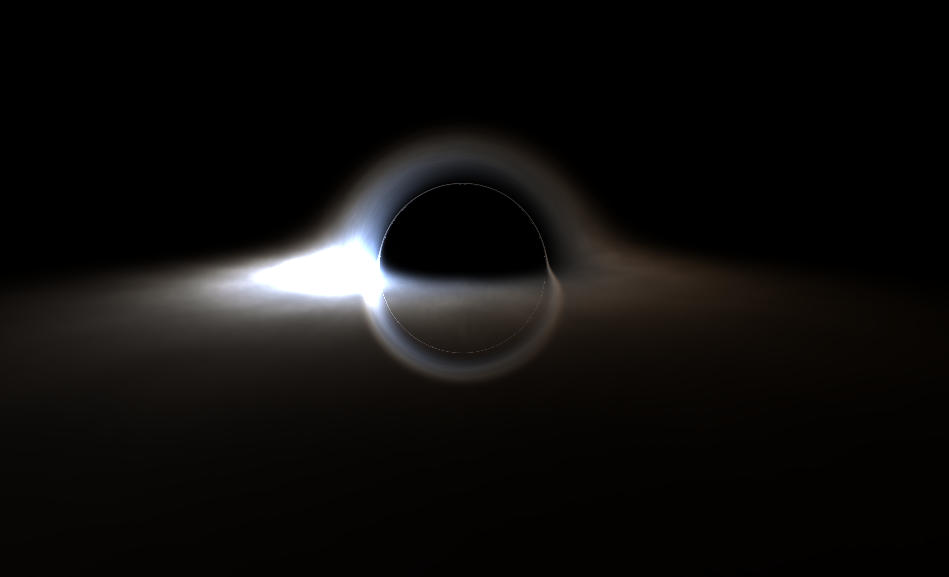
\includegraphics[width=0.95\textwidth]{photo/gb2.png}
            \caption{效果图3(高温,双多普勒)}
        \end{minipage}
        \hfill
        \begin{minipage}[t]{0.48\textwidth}
            \centering
            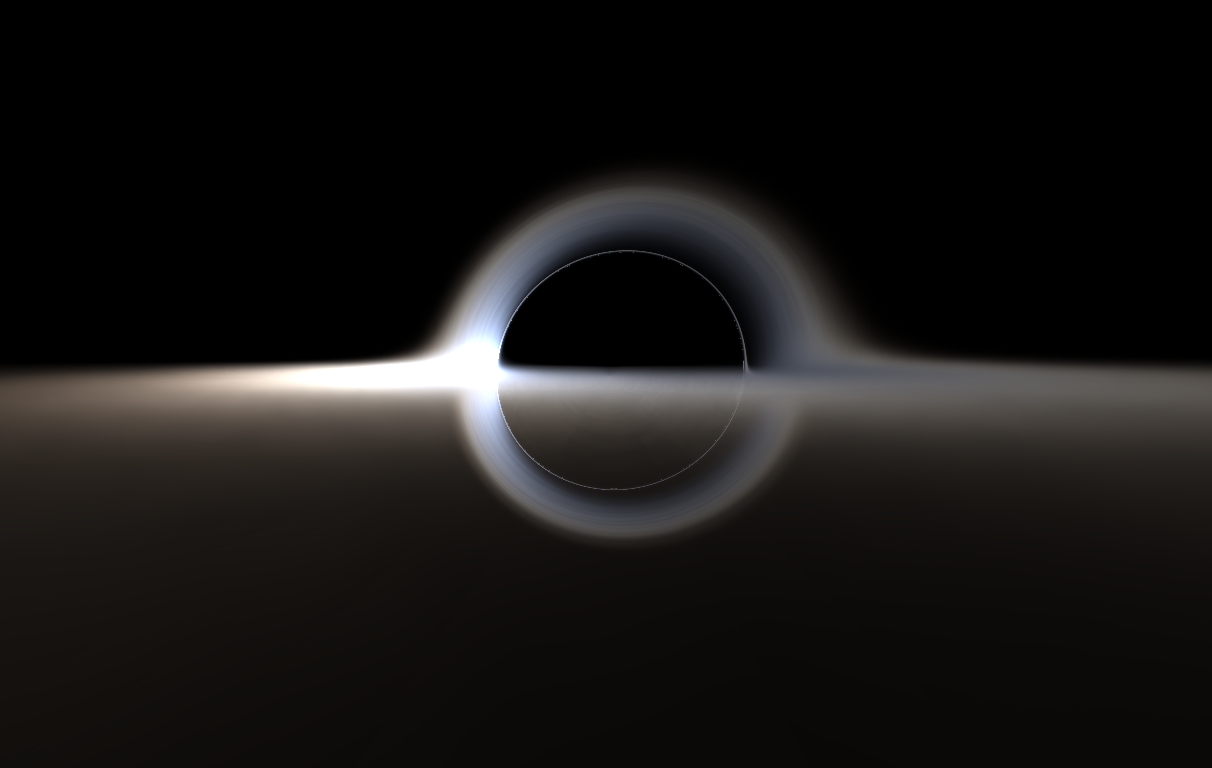
\includegraphics[width=0.95\textwidth]{photo/gb3.png}
            \caption{效果图4(高温,双多普勒)}
        \end{minipage}
    \end{figure}
    \subsection{参数可调、旋转吸积盘}
    之前的工作都是在固定参数下进行的,想改效果只能从源码修改,且渲染很长时间(主要花在光线步进)后
    只能得到一张图。现在我将ImGui引入程序,实现可调参数。并且通过将时间传入shader的方法实现让每帧
    吸积盘呈现旋转样式,让图变成动画。
    \begin{figure}[H]
        \centering
        % 第一行
        \begin{minipage}[t]{0.48\textwidth}
            \centering
            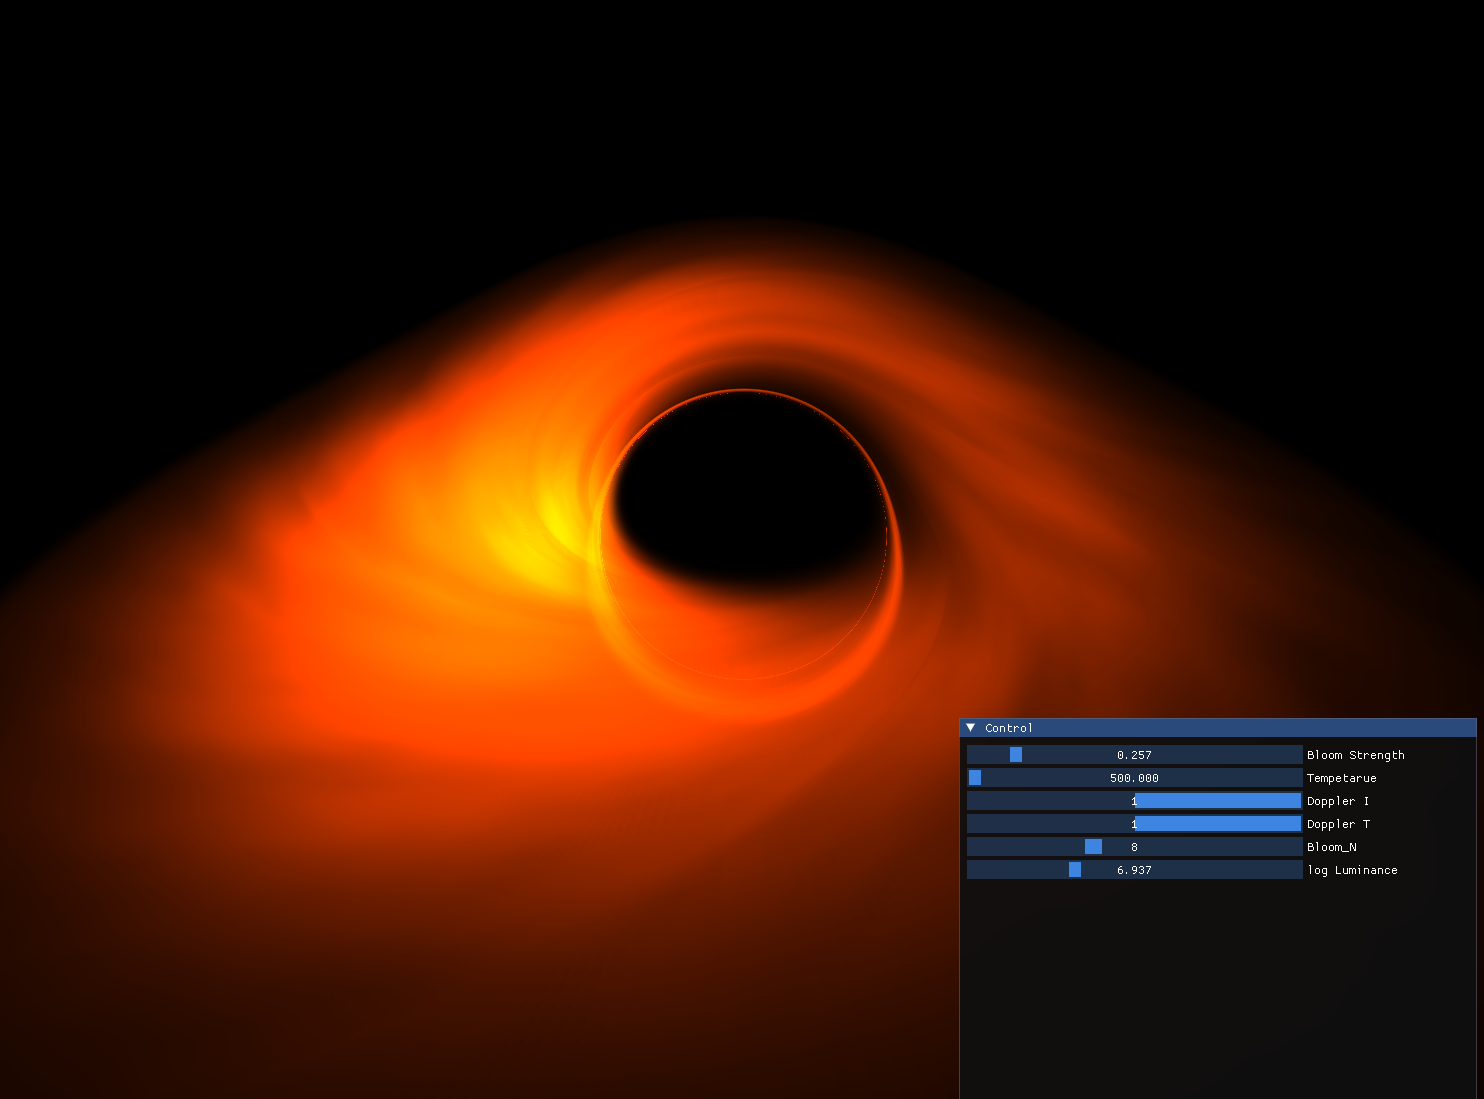
\includegraphics[width=1.03\textwidth]{photo/swz1.png}
            \caption{效果图1}
        \end{minipage}
        \hfill
        \begin{minipage}[t]{0.48\textwidth}
            \centering
            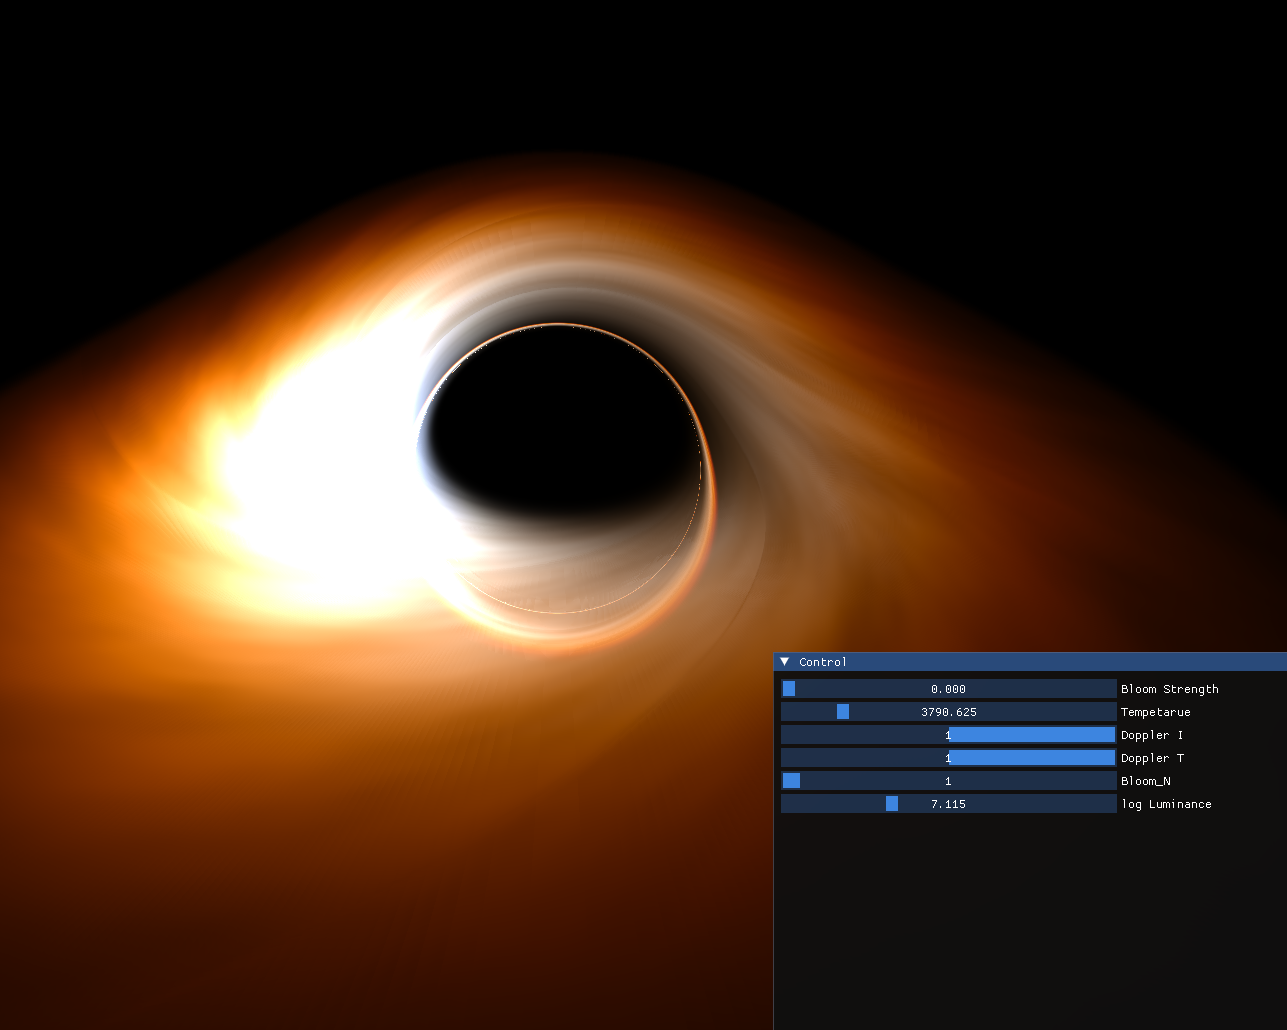
\includegraphics[width=0.95\textwidth]{photo/swz0.png}
            \caption{效果图2}
        \end{minipage}
    \end{figure}
    \subsection{Kerr黑洞、其他时空}
    《星际穿越》电影中的黑洞是一个旋转的黑洞(Kerr黑洞),因此我决定实现Kerr黑洞的渲染。
    使用sympy符号化计算导出了Kerr时空的64个联络,之后用笛卡尔坐标系光线步进。得到一系列图:
    \begin{figure}[H]
        \centering
        % 第一行
        \begin{minipage}[t]{0.48\textwidth}
            \centering
            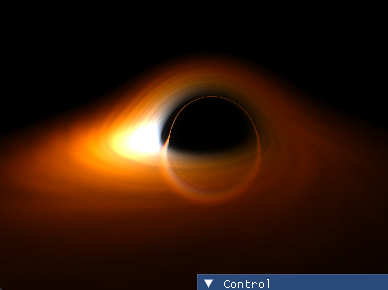
\includegraphics[width=0.95\textwidth]{photo/2k5T.png}
            \caption{温度参量2500K,黑洞自旋a=0.9}
        \end{minipage}
        \hfill
        \begin{minipage}[t]{0.48\textwidth}
            \centering
            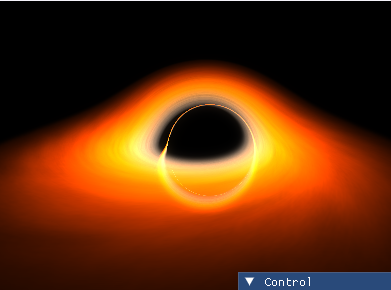
\includegraphics[width=0.95\textwidth]{photo/2k5T_ND.png}
            \caption{温度参量2500K,黑洞自旋a=0.9(无多普勒)}
        \end{minipage}
        \begin{minipage}[t]{0.48\textwidth}
            \centering
            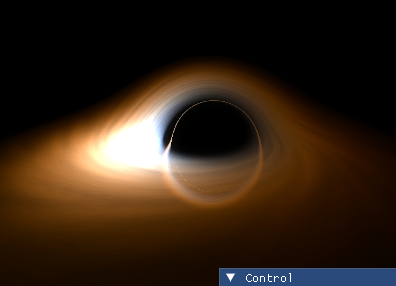
\includegraphics[width=0.95\textwidth]{photo/6kT.png}
            \caption{温度参量6000K,黑洞自旋a=0.9}
        \end{minipage}
        \hfill
        \begin{minipage}[t]{0.48\textwidth}
            \centering
            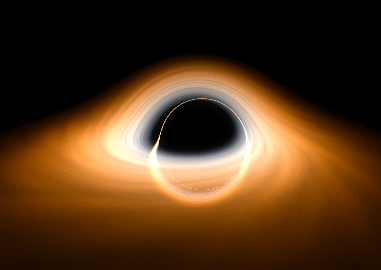
\includegraphics[width=0.95\textwidth]{photo/6kT_ND.png}
            \caption{温度参量6000K,黑洞自旋a=0.9(无多普勒)}
        \end{minipage}
        \begin{minipage}[t]{0.48\textwidth}
            \centering
            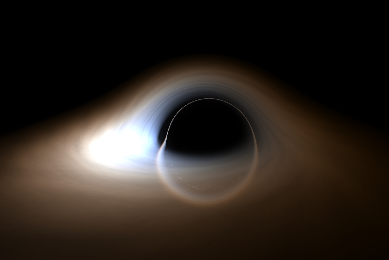
\includegraphics[width=0.95\textwidth]{photo/10kT.png}
            \caption{温度参量10000K,黑洞自旋a=0.9}
        \end{minipage}
        \hfill
        \begin{minipage}[t]{0.48\textwidth}
            \centering
            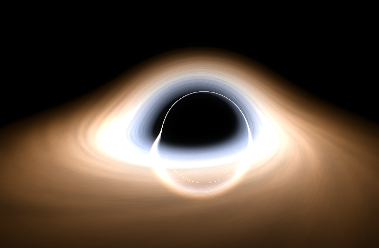
\includegraphics[width=0.95\textwidth]{photo/10kT_ND.png}
            \caption{温度参量10000K,黑洞自旋a=0.9(无多普勒)}
        \end{minipage}
        \begin{minipage}[t]{0.48\textwidth}
            \centering
            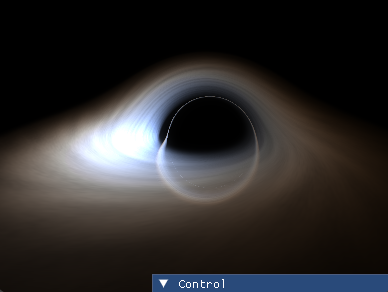
\includegraphics[width=0.95\textwidth]{photo/14kT.png}
            \caption{温度参量14000K,黑洞自旋a=0.9}
        \end{minipage}
        \hfill
        \begin{minipage}[t]{0.48\textwidth}
            \centering
            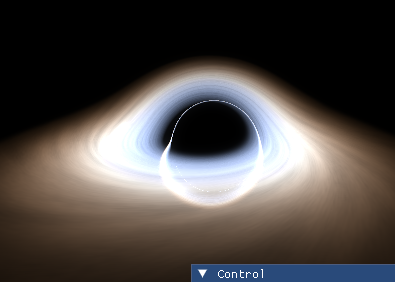
\includegraphics[width=0.95\textwidth]{photo/14kT_ND.png}
            \caption{温度参量14000K,黑洞自旋a=0.9(无多普勒)}
        \end{minipage}
    \end{figure}
    以下是我的黑洞渲染器的结果,于《星际穿越》中的卡冈图雅黑洞进行对比。差异
    主要在泛光强度、吸积盘噪声设置、吸积盘温度设置。
    \begin{figure}[H]
        \centering
        % 第一行
        \begin{minipage}[t]{0.48\textwidth}
            \centering
            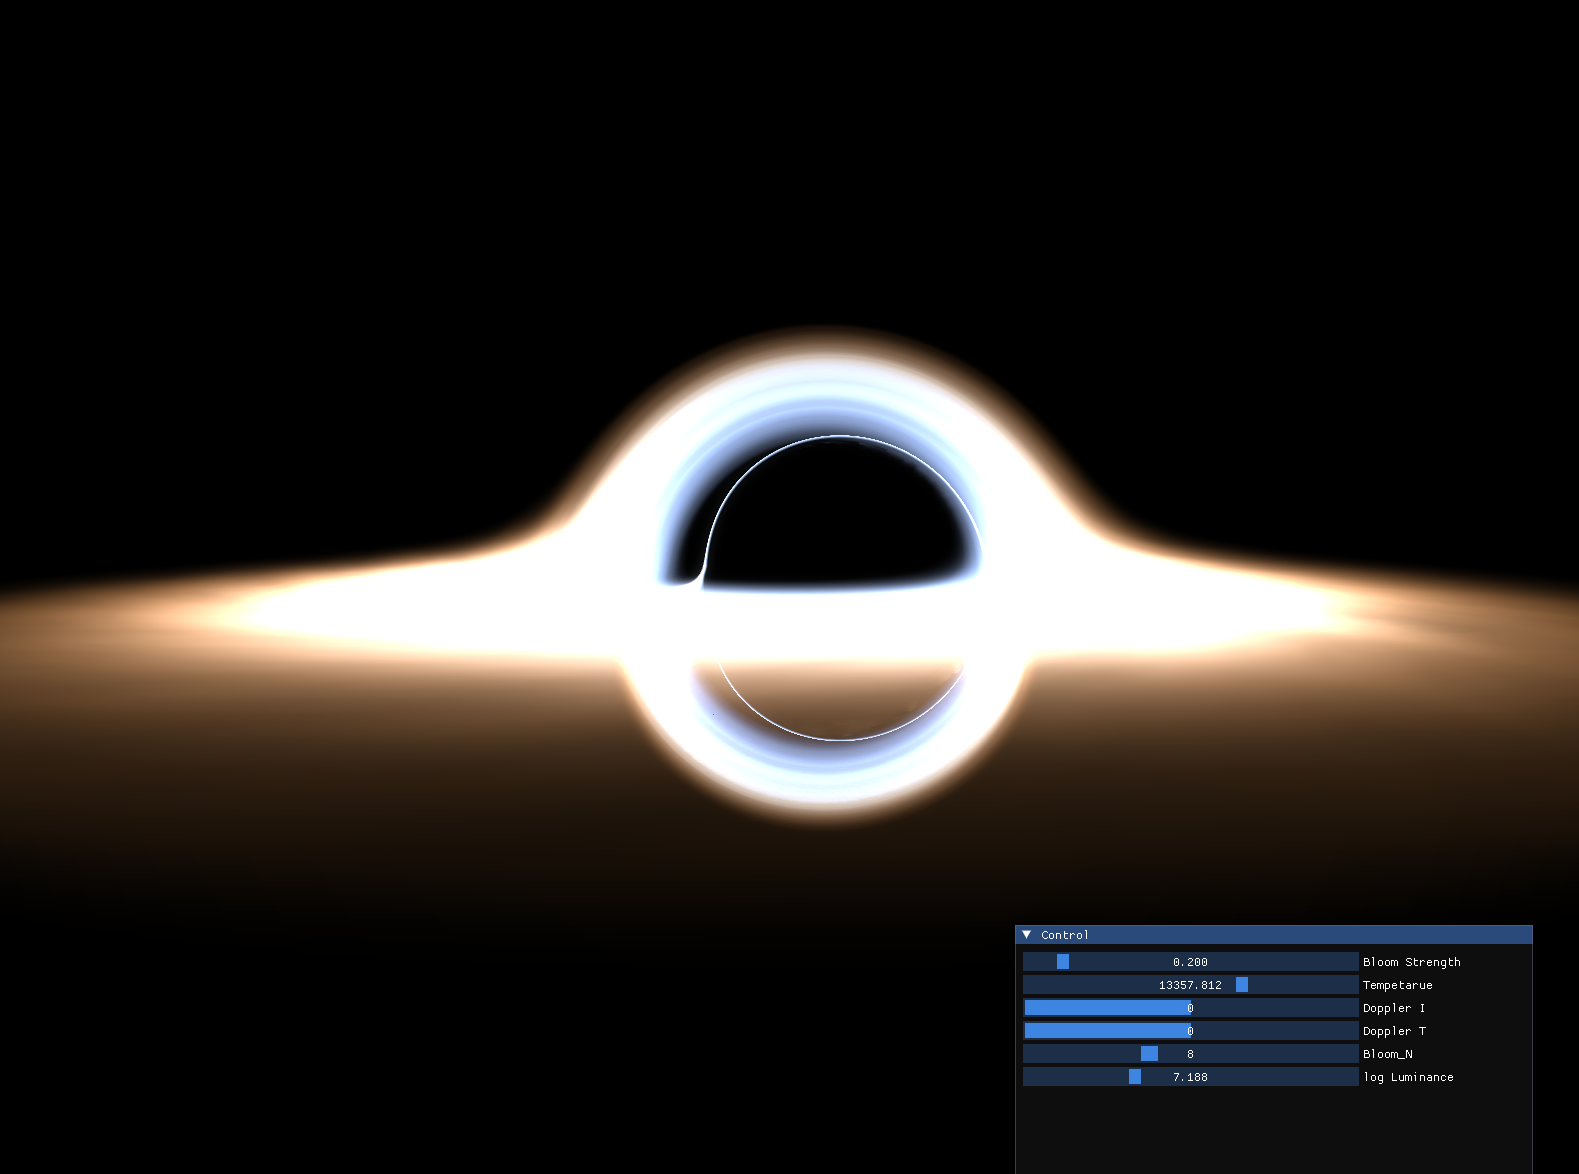
\includegraphics[width=0.95\textwidth]{photo/20k_2_ND.png}
            \caption{本渲染器:13500K,a=0.9,无多普勒}
        \end{minipage}
        \hfill
        \begin{minipage}[t]{0.48\textwidth}
            \centering
            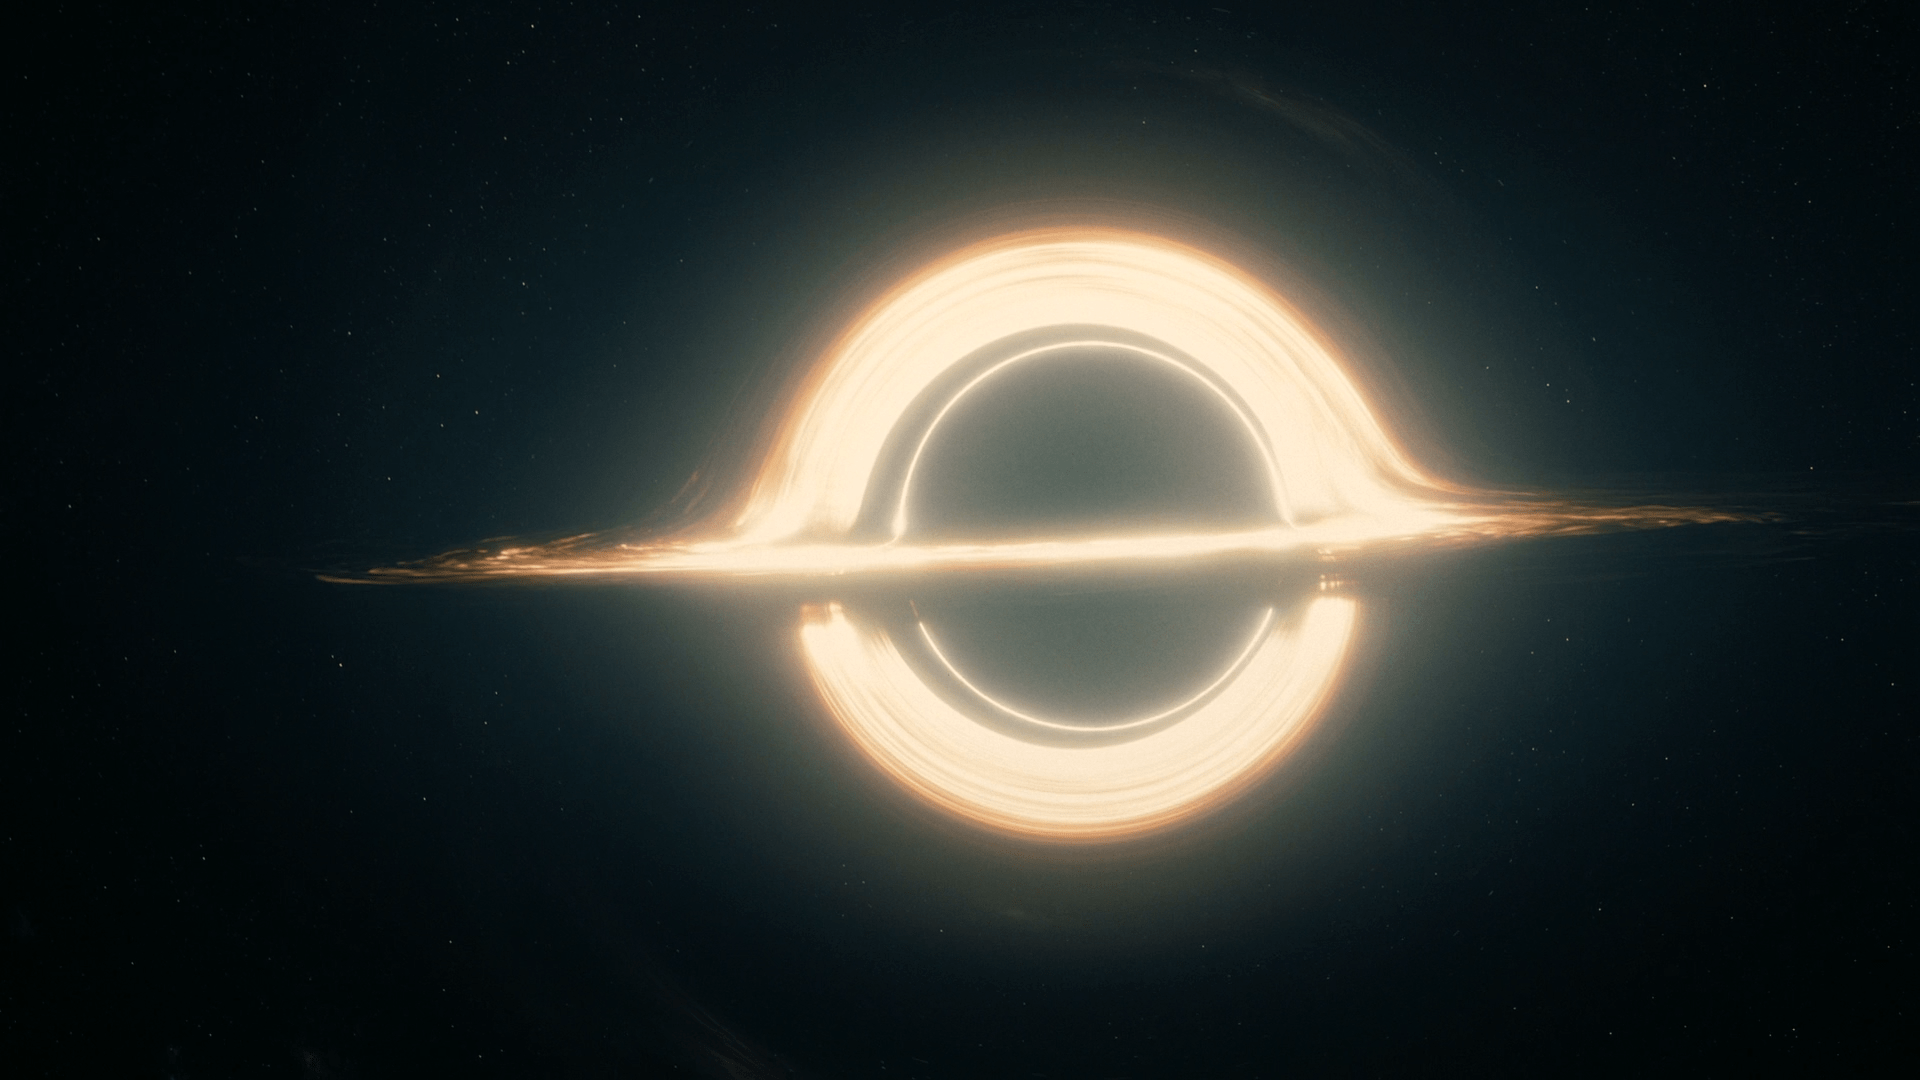
\includegraphics[width=0.95\textwidth]{photo/S.png}
            \caption{星际穿越:温度自旋未知,无多普勒}
        \end{minipage}
    \end{figure}
    为提升视觉效果的下一步工作:更改吸积盘噪声、增加外圈物质吸收率。\par
    原则来说带电黑洞的渲染也可以实现,但由于其形式和施瓦西黑洞类似,视觉效果也应当相近,这里没有实现。\par
    此外,我还测试了两个目前在物理上被认为不可能出现于宇宙中的时空:\par
    \begin{figure}[H]
        \centering
        % 第一行
        \begin{minipage}[t]{0.48\textwidth}
            \centering
            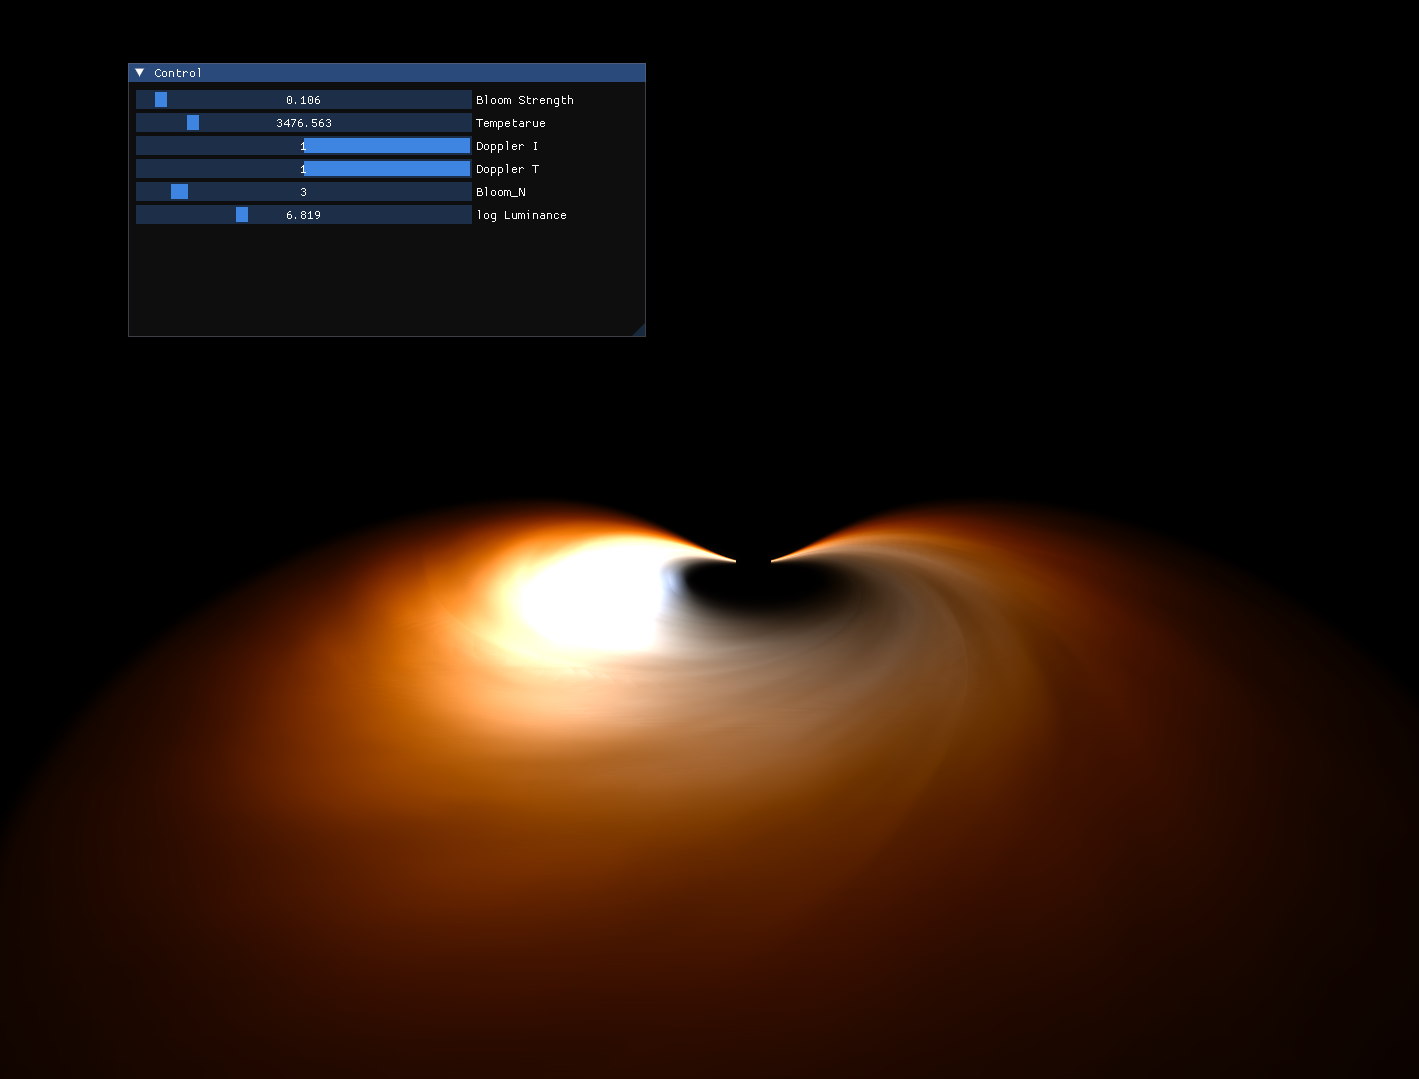
\includegraphics[width=0.95\textwidth]{photo/ip0.png}
            \caption{负质量施瓦西“黑洞”}
        \end{minipage}
        \hfill
        \begin{minipage}[t]{0.48\textwidth}
            \centering
            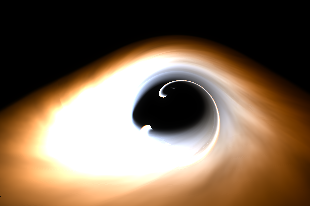
\includegraphics[width=0.95\textwidth]{photo/ip1.png}
            \caption{自旋大于1的Kerr黑洞,自旋a=1.5}
        \end{minipage}
    \end{figure}
    1.其是负质量,这意味着其会对光线进行排斥,这也是为什么其顶上会出现一个楔形黑色区域:发射向那里的光都被排斥到吸积盘外。\par
    2.其是自旋>1的黑洞,原则上会出现裸露的奇点。不过由于光线步进速度较慢以及设置保护性的截断(防止对负数开跟、分母由正向负突变),目前其
    中心的细节需要进一步改进。
    \section{下一步工作}
    \subsection{GPU并行光线步进}
    目前由于封装和简单考虑,光线步进程序仍然是串行/CPU并行(提升不高,约30\%)的。下一步工作是将光线步进程序并行化,尝试
    进行实时渲染(可变摄像机位置)。
    \subsection{吸积盘噪声更改}
    目前的噪声细节度不太够,下一步工作是将噪声细节度提升到更高的水平,达成更好的视觉效果。
    \subsection{辐射-RGB转换}
    目前的RGB转换是直接基于经验公式给出的,下一步工作是将其改为基于辐射强度的转换(即将辐射强度转换为XYZ坐标系下的颜色,再转换为RGB)。
    \subsection{其他时空}
    目前的工作仅限于施瓦西黑洞和Kerr黑洞,下一步工作是实现其他时空下的测地线计算(如Reissner-Nordström黑洞、Kerr-Newman黑洞等)。
    并观测更多非物理的时空。
    \subsection{说明文档完善、可移植性、轻量化}
    目前的说明文档较为简陋,下一步工作是完善说明文档、使其更易于阅读。
    另外,当前的代码并不易于移植(需要用户用CMake配置、编译),而且有部分参数必须在程序中调试。
    那么之后要使其更易于移植(如使用CMake配置文件)。甚至可以考虑将其打包为一个可执行文件。
    此外,应该把测试中的GSL去掉,其存储占用了40MB左右的空间,且GSL的使用并不多。GLM更是没有用到,也可以考虑删除。
\end{document}